\begin{figure*}
    \centering
    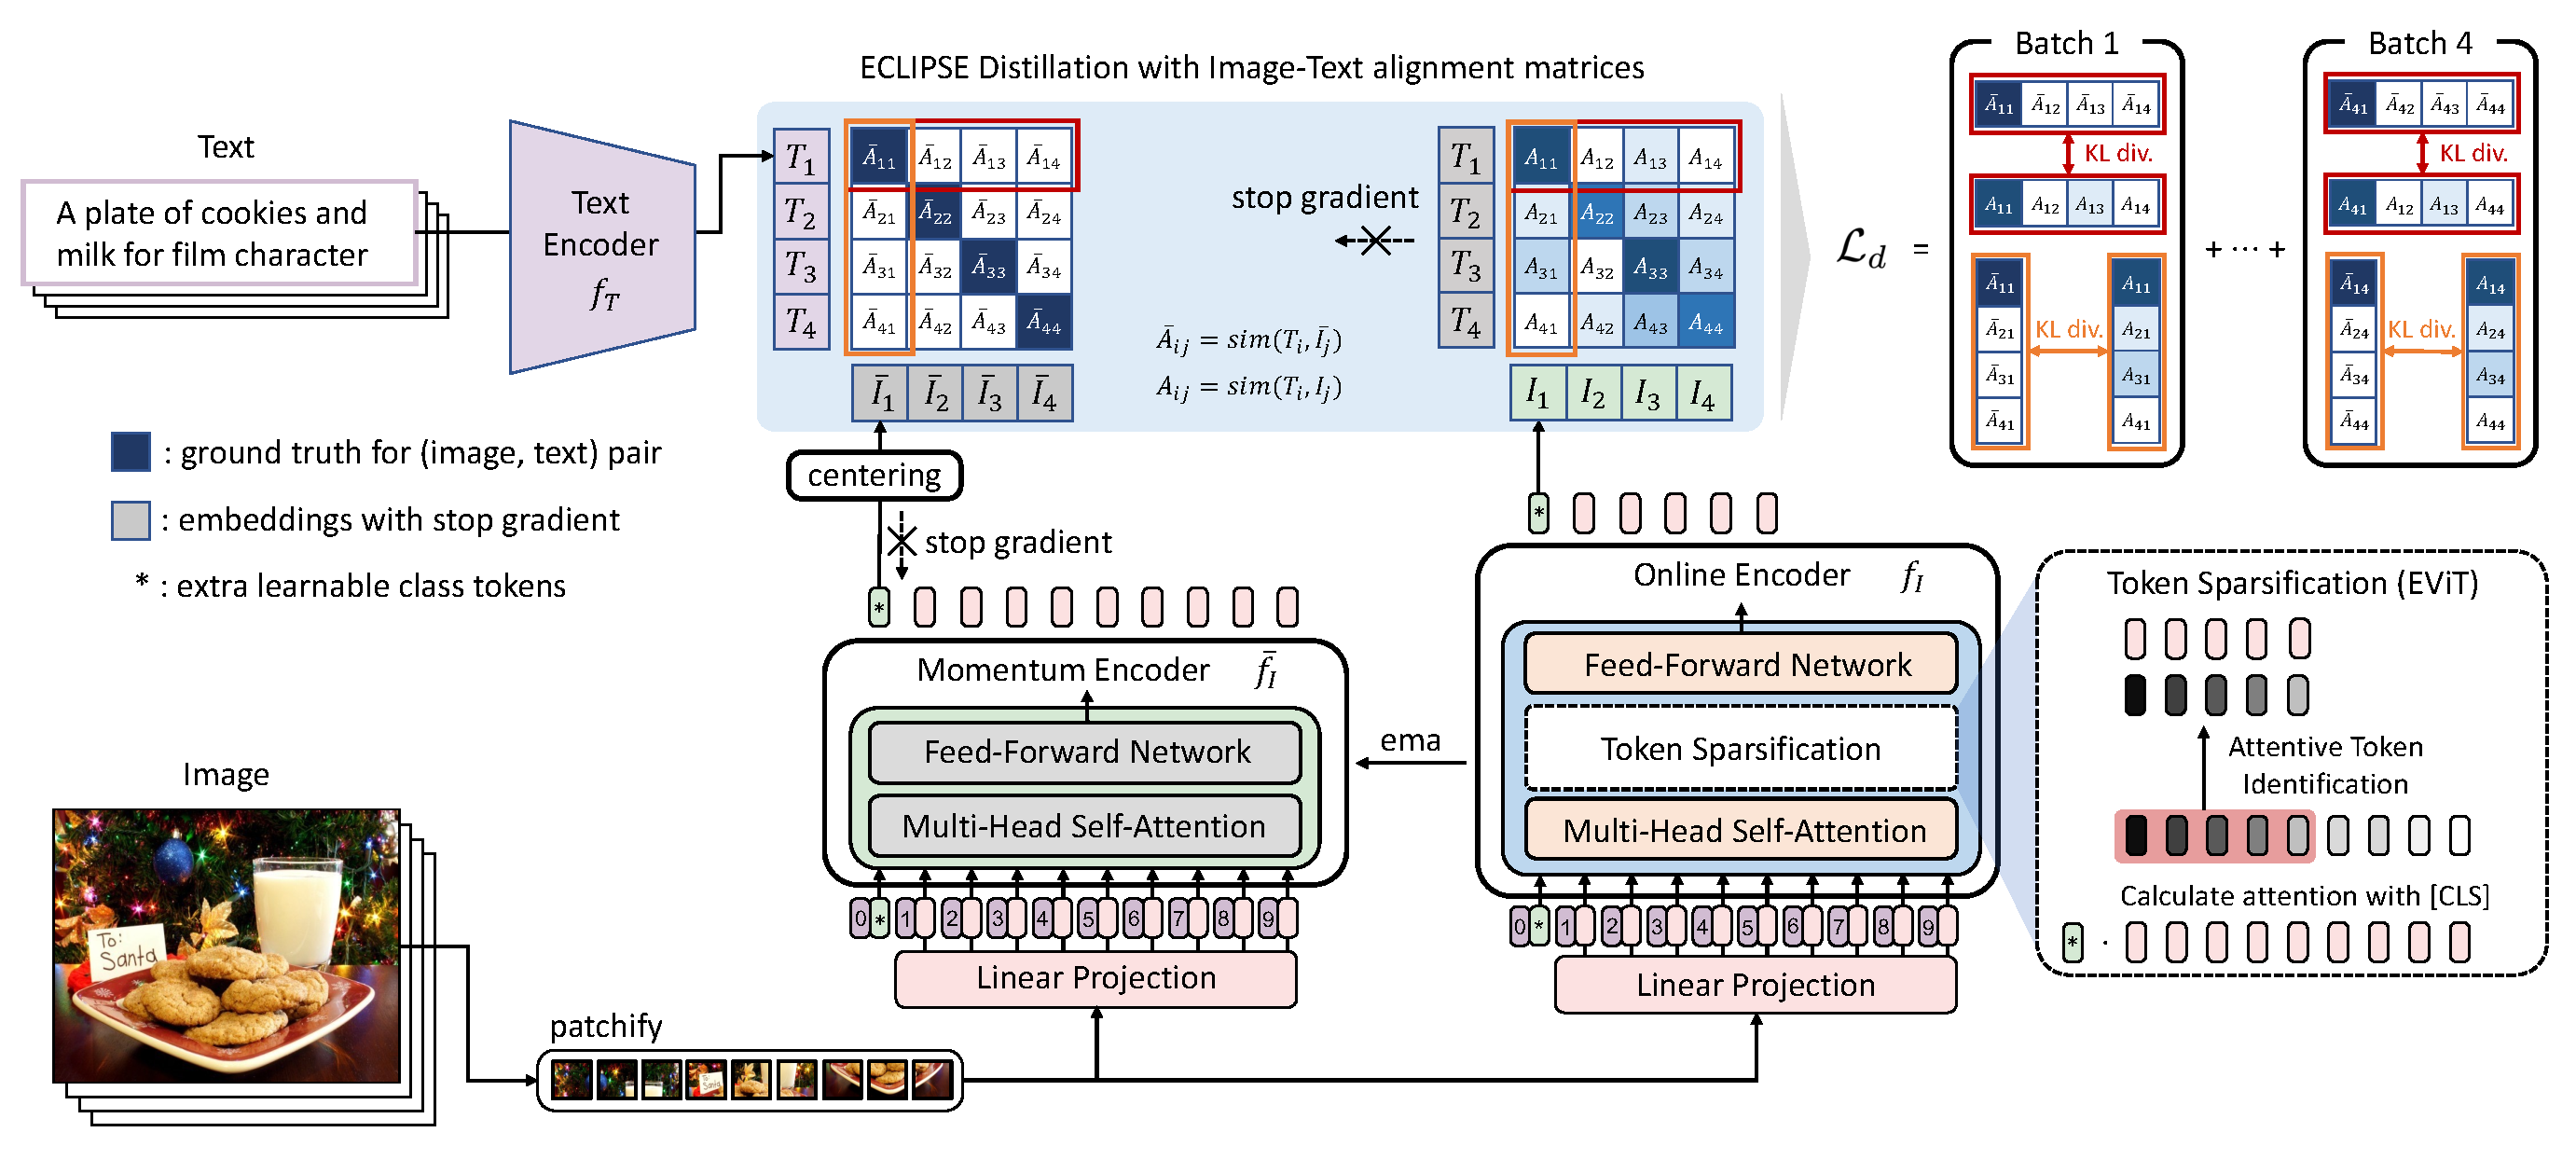
\includegraphics[width=0.9\textwidth]{figures/imgs/figure_overall.pdf}
    \caption{Overview of our proposed ECLIPSE. ECLIPSE is a meta-architecture for contrastive language-image pretraining that features a text encoder $f_T$, a momentum teacher encoder (Full ViT, $\bar{f}_I$), and a streamlined online encoder (ViT with token sparsification, $f_I$). Though the online network of ECLIPSE is compatible with any ViT acceleration method in literature~\cite{liang2022evit,rao2021dynamicvit,liang2022expediting}, we choose EViT~\cite{liang2022evit} due to its simple architecture without introducing additional parameters. Full ViTs without any sparsification can be also adopted for the online network, in which ECLIPSE then provides a full-capacity model with enhanced performance.
    }
    \label{fig:fig_architecture}
\end{figure*}
\section{Method}
\label{sec:method}

In this section, we propose ECLIPSE: Expediting Contrastive Language-Image Pretraining with Self-distilled Encoders.
Our goal is to resolve image-text misalignment problem of Contrastive Language-Image Pretraining (i.e., CLIP) for uncurated image-text pairs via efficient distillation formulation without extra text momentum encoder.
We further compensate the heavy computational cost of distillation by adopting model expediting~(i.e., EViT) to the online encoder that requires gradient computation.
We start from revisiting basic concepts of CLIP and EViT~\cite{liang2022evit}.
Then, we introduce our meta-architecture ECLIPSE that combines CLIP with our novel knowledge distillation structure and ViT acceleration for efficient training and inference.

\subsection{Contrastive Language-Image Pre-training}

First, we revisit basic form of contrastive language--image pretraining~\cite{radford2021learning}.
CLIP features a dual-encoder architecture where the image encoder $f_I$ and text encoder $f_T$ are jointly trained with contrastive objective $\mathcal{L}_{C}$.

\paragraph{Image-Text Alignment Matrix.}
For convenience, we denote $A\in\mathbb{R}^{N\times N}$ as the image-text alignment matrix for a given batch of $N$ image-text pairs $\{(x_i^I,x_i^T)\}_{i=1}^N$.
Each element of the image-text alignment matrix $A_{ij}$ is the cosine similarity between the projected representations of the $i$-th text and $j$-th image (i.e., $T_i=f_T(x^T_i)$ and $I_j=f_I(x^I_j)$, respectively), written as:
\begin{equation}
\label{eq:align}
    A_{ij}=\mbox{sim}(T_i, I_j), %~\bar{A}_{i,j}=\mbox{sim}(T_i, \bar{I}_j), 
\end{equation}
where sim$(\cdot)$ is cosine similarity.

\paragraph{InfoNCE Loss.}
In CLIP, the encoded image features $I$ and text features $T$ are projected to the same dimension where the embeddings for matching image-text pairs are pulled together while embeddings for non-matched pairs are pushed apart with the InfoNCE loss~\cite{oord2018representation}.
Using Eq.~(\ref{eq:align}), the InfoNCE loss $\mathcal{L}_N$ is rewritten as:
\begin{equation}
\label{eq:infoNCE}
    \mathcal{L}_{N}(A)=-\frac{1}{N}\sum_{i=1}^N\log{\frac{\exp{\big(A_{ii}/\tau\big)}}{\sum_{j=1}^N\exp{\big(A_{ij}/\tau\big)}}},
\end{equation}
where $\tau$ is a learnable temperature variable.
The loss for the text encoder $\mathcal{L}_{T}$ and image encoder $\mathcal{L}_{I}$ are written as:
\begin{equation}
\label{eq:CLIP}
    \mathcal{L}_{T}= \mathcal{L}_{N}(A), ~~\mathcal{L}_{I}= \mathcal{L}_{N}(A^T).
\end{equation}
The overall loss for CLIP is the average of the loss for each encoder, written as $\mathcal{L}_{\text{CLIP}}(A)=\frac{1}{2}(\mathcal{L}_T+\mathcal{L}_I)$.

\subsection{Accelerating ViTs with Token Sparsification}
Previous work in ViT acceleration~\cite{rao2021dynamicvit,liang2022evit} mainly focused on token sparsification since the complexity of transformer attention is reduced at a quadratic scale with respect to the number of tokens that are discarded, significantly improving model throughputs.
Most recent works proposed token sparsification via external models or reorganizing the patch tokens based on their attentiveness with the \texttt{[CLS]} token.
In this work, we benchmark EViT~\cite{liang2022evit} since no additional parameters are introduced for acceleration.
We follow their architecture design and discard a fixed ratio ($1$-$\kappa$) of inattentive tokens according to the attention value between the \texttt{[CLS]} token and each patch in the $4^{th}$, $7^{th}$, and $10^{th}$ transformer layers, where $\kappa$ is the token keep rate.

\subsection{ECLIPSE}
Towards a data-efficient pretraining with uncurated image-text pairs, we propose ECLIPSE, a novel distillation pipeline that alleviates image-text misalignments.
The overall architecture of ECLIPSE is illustrated in Figure~\ref{fig:fig_architecture}.
ECLIPSE features a text encoder, a online image encoder (EViT), and a momentum encoder (ViT).
Below we provide a step-by-step description of our proposed ECLIPSE architecture.

\paragraph{Knowledge Distillation.}
Knowledge distillation, introduced by~\cite{hinton2015distilling}, is a learning paradigm where we train the student network to mimic the ``soft" labels predicted from the teacher network.
Following previous intuition, we adopt a knowledge distillation framework for the token-sparsified online ViT (student) to train the output of the full ViT with momentum weights (teacher), aiming to accelerate ViT without degrading performance.
However, our empirical results show that applying conventional distillation~\cite{hinton2015distilling,touvron2021training,caron2021emerging} (i.e., training the student network to directly predict the output of the teacher network) to CLIP shows minor improvement in performance when transferred to downstream tasks. %(see Sec.~\ref{subsec:ablation}).
Motivated by this finding, we propose a unique distillation architecture via the image-text alignment matrices denoted in Eq.~(\ref{eq:align}).

\paragraph{Training Loss of ECLIPSE.}
Given the momentum encoder $\bar{f}_I$, online encoder $f_I$ and text encoder $f_T$, we define a pair of alignment matrices using Eq.~(\ref{eq:align}) as:
\begin{equation}
    \bar{A}_{ij}=\mbox{sim}(T_i, \bar{I}_j), ~~A_{ij}=\mbox{sim}(\text{sg}(T_i), I_j),
\end{equation}
where $\text{sg}$ denotes stop-gradient and $\bar{I}_j=\bar{f}_I(x^I_j)$, $I_j=f_I(x^I_j)$ is the projected representations of $j$-th image with the momentum encoder and online encoder, respectively.
Note that gradient is not calculated for the momentum encoder $\bar{I}$ as it is updated by EMA of the online encoder $I$.

We first obtain the loss for the teacher-text alignment matrix $\bar{A}$ with InfoNCE loss in Eq.~(\ref{eq:infoNCE}), denoted as $\mathcal{L}_{\text{CLIP}}(\bar{A})$.
Instead of training the online network to directly predict the output of the momentum network, we distill knowledge by predicting $A$ to match $\bar{A}$.
We define the distillation loss with KL divergence for each row and column between two matrices.
Let $\sigma$ be the softmax function, the KL divergence between $A$ and $\bar{A}$ is rewritten as:
\begin{equation}
    D_{\text{KL}}(\bar A||A) = \sum_{i=1}^N \sigma(\bar A_i) \log \frac{\sigma(A_i)}{\sigma(\bar A_i)}.
\end{equation}
The overall distillation loss is the average of KL loss for row vectors and column vectors, written as $\mathcal{L}_{\text{distill}}(\bar{A},A)=\frac{1}{2}(D_{\text{KL}}(\bar A|| A) + D_{\text{KL}}(\bar A^T|| A^T))$.

To accelerate training for the online network, we balance $\mathcal{L}_{\text{distill}}$ with InfoNCE loss $\mathcal{L}_{\text{CLIP}}(A)$~\cite{touvron2021training}.
The final loss of the online network is then written as:
\begin{equation}
    \mathcal{L_{\text{online}}}=\lambda\mathcal{L}_{\text{CLIP}}(A)+(1-\lambda) \mathcal{L}_{\text{distill}}(\bar{A},A),
    \label{eq:distill}
\end{equation}
where $\lambda$ is a parameter that balances the KL divergence loss and the InfoNCE loss.
The final loss for ECLIPSE is then written as:
\begin{equation}
    \mathcal{L}=\mathcal{L}_{\text{online}}+\mathcal{L}_{\text{CLIP}}(\bar{A}).
\end{equation}

\paragraph{Momentum Update.}
Let $\theta_{f_I}$, $\theta_{\bar{f}_I}$ be the parameter of the online image encoder and momentum encoder, respectively.
For the $t$-th step, we update $\theta^{(t)}_{\bar{f}_I}$ of the momentum encoder according to the following:
\begin{equation}
    \theta_{\bar{f}_I}^{(t)} = m \theta_{\bar{f}_I}^{(t-1)} + (1-m) \theta_{f_I}^{(t)},
\end{equation}
where $m$ denotes the momentum parameter. We use $m=0.994$ in our experiments.
Momentum centering is also adopted for $\bar{f}_I$~\cite{caron2021emerging} (see our supplement for further discussion with regard to the momentum parameter and centering).